\chapter{Results}
\label{ch:results}

% sections
% 1 qualitative analysis (added by me)
% 2 setup
% 3 acquisition params
% 4 data treatment



% intro to results
This chapter presents the results of the thesis.
The results are divided into four parts: qualitative analysis, characterization of the setup, optimization of the acquisition parameters, and data treatment.
SE images of the analyzed areas are included the \hyperref[appendix:SE_images]{Appendix B}.


\brynjar{Legge til kommentar om SE at jeg har valgt homogene områder, i tillegg til å ta noen spektra fra scratched område.}



% 1 qualitative analysis
\section{Qualitative analysis}
\label{results:qualitative_analysis}

The qualitative analysis present general plots of the spectra, where the lines and the artifacts are identified.
Selected spectra are plotted in \cref{fig:results:overviewGaSb_withArtifacts,fig:results:GaSb_voltages,fig:results:GaAs_voltages}.
The y-axis have a logarithmic scale, and the x-axis have a linear scale.
The y-axis is the intensity of the signal, i.e. the number of counts in each channel.
The x-axis is the energy of the signal.
\cref{fig:results:overviewGaSb_withArtifacts} have annotated relevant information in the spectra.


% figures/results/spectrum_overview.pdf
\begin{figure}[hbtp]
    \centering
    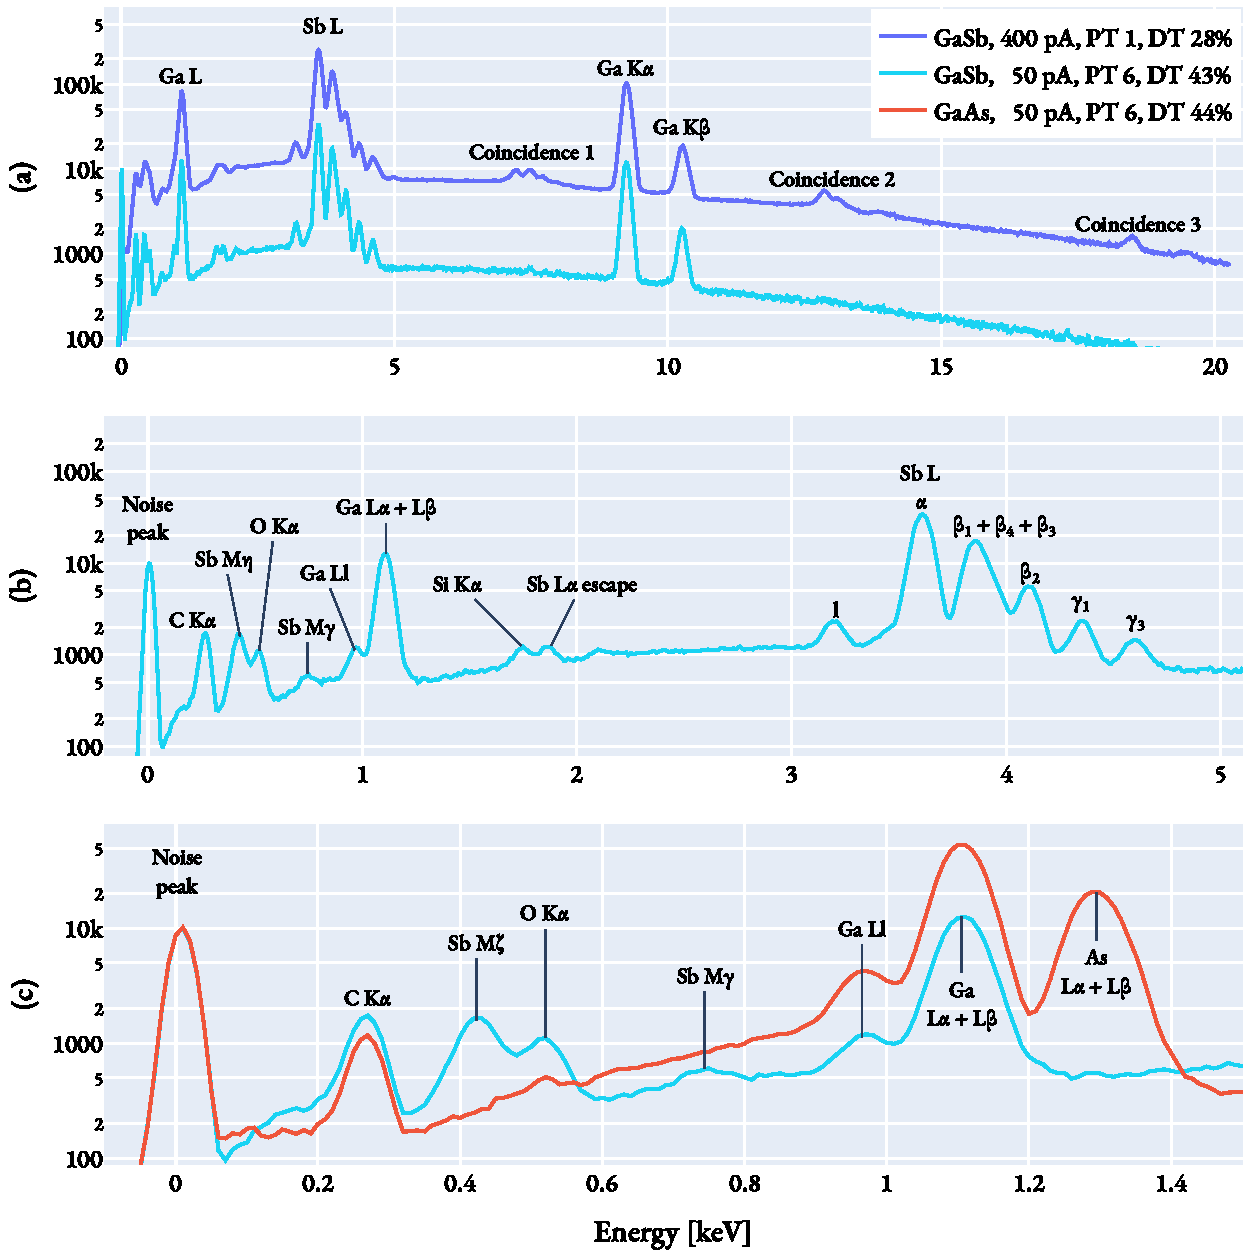
\includegraphics[width=0.99\linewidth]{figures/results/spectrum_overviews.pdf}
    \caption{
        Overview of the GaSb spectra.
        The blue line in panel (a) have lower resolution and more artifacts than the red line.
        The red line is plotted in panel (b) over a shorter energy range.
        Panel (c) show the red line on a even shorter energy range, with the GaAs spectrum in light blue for reference.
    }
    \label{fig:results:overviewGaSb_withArtifacts}
\end{figure}


% figures/results/GaSb_voltages.pdf
\begin{figure}[hbtp]
    \centering
    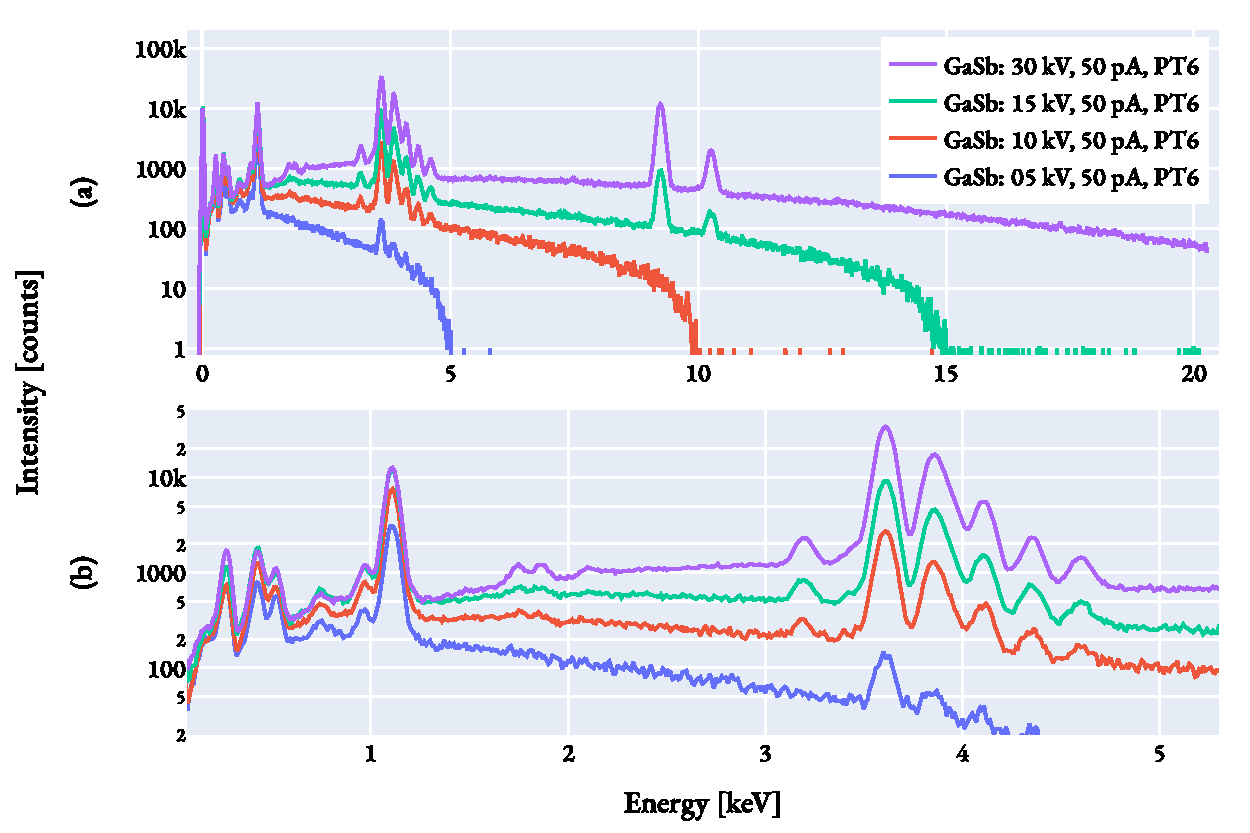
\includegraphics[width=0.90\linewidth]{figures/results/GaSb_voltages.pdf}
    \caption{
        The GaSb voltage series.
        Equal beam current and process time are used for all spectra.
    }
    \label{fig:results:GaSb_voltages}
\end{figure}


% figures/results/GaAs_voltages.pdf
\begin{figure}[hbtp]
    \centering
    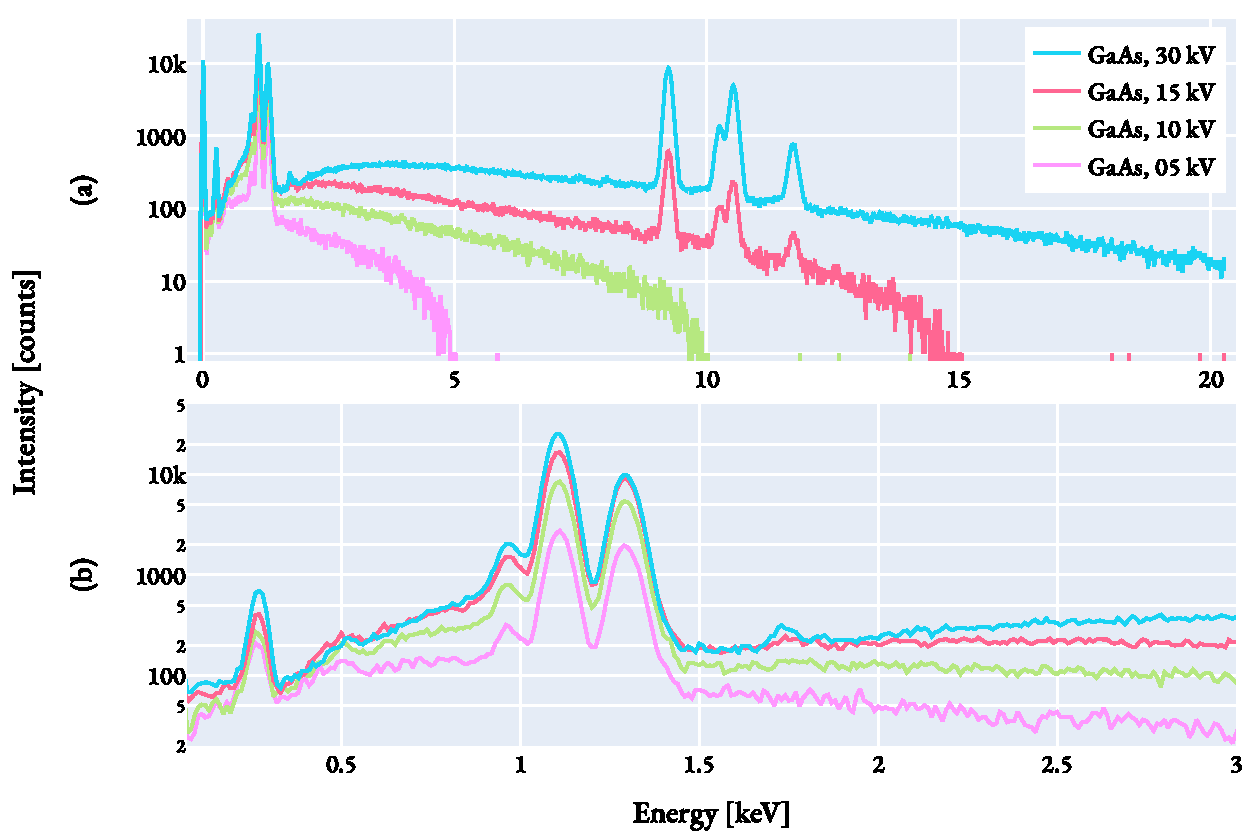
\includegraphics[width=0.90\linewidth]{figures/results/GaAs_voltages.pdf}
    \caption{
        The GaAs voltage series.
        Equal beam current and process time are used for all spectra.
    }
    \label{fig:results:GaAs_voltages}
\end{figure}



\subsection*{Lines}
\label{results:qualitative_analysis:lines}

All the lines given in \cref{tab:theory:lineEnergies} for Ga, As, and Sb have been identified in the spectra.
All spectra also had a peak at C K$\alpha$.
The GaSb spectra included a O K$\alpha$ peak.
As annotated in \cref{fig:results:overviewGaSb_withArtifacts}, the GaSb spectra also included two Sb M-peaks: $\eta$ and $\gamma$.
These two M-peaks are not listed in the HyperSpy database, but were found through AZtec \cite{aztec_manual} and other literature \cite{liao2006practical}.




% the missing M-lines in HS, which were identified with AZtec.


\subsection*{Artifacts}
\label{results:qualitative_analysis:artifacts}

Artifacts are present in all spectra, in varying degrees.
The artifacts identified are listed and described in \cref{tab:results:artifacts}.
The artifacts present in the spectra are the background, the noise peak, the carbon and oxygen stray peak, coincidence peaks, the internal Si fluorescence peak, and the Si escape peak from Sb La.

% The background is present in all spectra, and with increasing background intensity with higher count rates.
% The effect of a strong absorption edge which reduce the background intensity above its energy is most prominent in the GaAs spectra.
% Here it is the absorption edge in the L-peaks which reduce the background intensity abruptly above the L-peaks.
% Coincidence peaks are only present in some spectra, and are most prominent in the spectra with very high count rates.
% The spectra with beam energy 5, 10, and 15 keV also show coincidence events above E$_0$, e.g. visible in panel (a) in \cref{fig:results:GaSb_voltages}.


\begin{table}[phtb]
	\begin{center}
		\caption{
			The artifacts present in the spectra.
			See \cref{fig:results:overviewGaSb_withArtifacts,fig:results:GaSb_voltages,fig:results:GaAs_voltages}.
		}
		\renewcommand*{\arraystretch}{1.4}
		\label{tab:results:artifacts}
		\begin{tabular}{p{3.5cm}p{11.1cm}}
			\hline
			\textbf{Artifact}                                & \textbf{Where the articat is present and a comment}                                                                                                                                                                                                                                                                                                                                                                                             \\
			\hline
			Background                                       & All spectra. Increase with higher count rate.                                                                                                                                                                                                                                                                                                                                                                                                   \\
			Absorption edge effect on background             & Most prominent in GaAs. Reduces the background intensity above the Ga L absorption edge. In \cref{fig:results:GaAs_voltages} panel (b) the background drop from around 600 to around 170 counts.                                                                                                                                                                                                                                                \\
			Noise peak                                       & All spectra. Located almost at 0 keV.                                                                                                                                                                                                                                                                                                                                                                                                           \\
			Coincidence peaks                                & Only the spectra with very high count rates. \cref{fig:results:overviewGaSb_withArtifacts} with GaSb taken at 30 kV, 400 pA, and PT1 show coincidence peaks from: (Sb L + Sb L), (Sb L + Ga K), and (Ga K + Ga K).                                                                                                                                                                                                                              \\
			Tailing background noise from coincidence events & Present in spectra taken at 5, 10, and 15 kV. Coincidence events from two arbitrary counts give a tailing background. Exemplified by the green 15 kV line in \cref{fig:results:GaSb_voltages} panel (a), where vertical lines (one count each) are present between 15 and 20 keV.                                                                                                                                                               \\
			Internal fluorescence peak                       & Visible in some spectra. A low signal, barely a peak in some spectra, at Si K$\alpha$.                                                                                                                                                                                                                                                                                                                                                          \\
			Si escape peak                                   & Most GaSb spectra show some escape signal from Sb L$\alpha$ at 1.86 keV, labeled in \cref{fig:results:overviewGaSb_withArtifacts} panel (b). The coincidence counts from (Sb L + Sb L) marked as "Coincidence 1" in \cref{fig:results:overviewGaSb_withArtifacts} panel (a) has one peak at 7.2 keV and one at 7.5 keV, where the latter cound be a combination of coincidence events and escape counts from Ga K$\alpha$ (9.25 - 1.74 = 7.51). \\
			Stray C                                          & All spectra show a C K$\alpha$ peak, with some variation in intensity.                                                                                                                                                                                                                                                                                                                                                                          \\
			Stray O                                          & All spectra of GaSb show an O K$\alpha$ peak. The GaAs spectra have much lower, but still present signal at 0.52 keV.                                                                                                                                                                                                                                                                                                                           \\
			\hline
		\end{tabular}
	\end{center}
\end{table}



























% 2 setup
\section{Characterization of the setup}
\label{results:setup}

The parameters of the setup are: energy resolution, the energy scale and offset, peak ratios, and deviations in peak positions.



\subsection*{Energy resolution of the detector}
\label{results:setup:energy_resolution}

The energy resolution, as the FWHM of the estimated or calculated Mn K$\alpha$ peak, is both a function of the detector and the acquisition parameters.
The best energy resolution obtained was 124 eV for the GaSb spectra, and 127 eV for the GaAs spectra.
The data show that the energy resolution is dependent on both the process time and input count rate, where the input count rate change with beam current and beam energy.
As the acquisition parameters affect the energy resolution, the energy resolutions listed in \cref{tab:results:energy_resolutions} are given with the relevant acquisition parameters.
All the values are given as the FWHM of the Mn K$\alpha$ peak, which is calculated with \cref{eq:estimateFWHM} through HyperSpy.
Specifying a single energy resolution for the detector should be accompanied by the acquisition parameters used to obtain the energy resolution, and by the method used to estimate the energy resolution.
Averaging the numbers have not been done as this neglects the effect of the acquisition parameters on the energy resolution.


\begin{table}[htbp]
    \begin{center}
        \caption{
            The energy resolutions [eV] in the different spectra.
            The table is sorted by process time, then ICR.
            All energy resolutions are calculated with \cref{eq:estimateFWHM}.
        }
        % \renewcommand*{\arraystretch}{1.4}
        \label{tab:results:energy_resolutions}
        \begin{tabular}	{p{1.5cm}ccrrr}
            \hline
            \textbf{		} & \textbf{	Energy resolution	} & \textbf{	PT	} & \textbf{	ICR	} & \textbf{	E$_0$	} & \textbf{	I$_\textnormal{beam}$	} \\
            \hline
                        & 158                          & 1             & 17000          & 30               & 50                               \\
                        & 158                          & 1             & 160000         & 30               & 400                              \\
                        & 143                          & 2             & 17000          & 30               & 50                               \\
                        & 132                          & 4             & 17000          & 30               & 50                               \\
                        & 128                          & 6             & 1080           & 5                & 50                               \\
            GaSb        & 127                          & 6             & 2300           & 10               & 50                               \\
                        & 125                          & 6             & 5700           & 15               & 50                               \\
                        & 127                          & 6             & 17000          & 30               & 50                               \\
                        & 127                          & 6             & 17000          & 30               & 50                               \\
                        & 124                          & 6             & 22000          & 15               & 200                              \\
                        & 125                          & 6             & 42000          & 15               & 400                              \\
            \hline
                        & 127                          & 6             & 880            & 5                & 25                               \\
                        & 127                          & 6             & 1750           & 10               & 25                               \\
            GaAs        & 129                          & 6             & 3300           & 15               & 25                               \\
                        & 128                          & 6             & 8000           & 30               & 25                               \\
                        & 129                          & 6             & 16400          & 30               & 50                               \\
            \hline
        \end{tabular}
    \end{center}
\end{table}



\subsection*{Energy scale and offset}
\label{results:setup:scale_offset}

The energy scale and offset are the parameters which are used to calibrate the spectra.
Both metrics are quite consistent between the spectra, and the energy scale match with the setting used in the acquisition (10 eV per channel).
The averaged values and the standard deviations are listed in \cref{tab:results:scale_offset}.
The calculated scale of the detector is equal to the instrument setting at 10 eV per channel, with very low standard deviation between the spectra at 0.04 eV/channel.
The zero offset was calculated to be -0.205 keV, which is a deviation of half a channel from the instrument setting of -0.2 keV.
The standard deviation of the offset is 0.004 keV.

% TODO: Comment that the std of the offset is one order of magnitude closer to the avg compared to the std vs avg of the scale.

\begin{table}[htbp]
    \begin{center}
        \caption{
            The scale and offset in the spectra.
        }
        \renewcommand*{\arraystretch}{1.2}
        \label{tab:results:scale_offset}
        \begin{tabular}{rrrrr}
            \hline
            \textbf{Samples}   & \textbf{Scale, average} & \textbf{Scale, std}  & \textbf{Offset, average} & \textbf{Offset, std} \\
                               & \emph{[keV/channel]}    & \emph{[keV/channel]} & \emph{[keV]}             & \emph{[keV]}         \\
            \hline
            Instrument setting & 0.010000                & -                    & -0.2000                  & -                    \\

            GaSb               & 0.010001                & 8.7E-06              & -0.2044                  & 4.4E-03              \\
            GaAs               & 0.010018                & 6.6E-05              & -0.2075                  & 4.9E-03              \\
            GaSb + GaAs        & 0.010007                & 3.8E-05              & -0.2054                  & 4.3E-03              \\
            \hline
        \end{tabular}
    \end{center}
\end{table}




\subsection*{Peak ratios}
\label{results:setup:peak_ratios}

The results from the peak ratios are listed in \cref{tab:results:peak_ratios}.
The peak ratios are useful to alert carbon contamination over time, and to identify and quantify stray radiation with certain sample geometry.
As the results are neither a series over time or taken with the required sample geometry, the results in the table are a demonstration of the metric without any further interpretation.
Peak ratios are also used for quantification, but needs bulk corrections.
The table show that some of the peak ratios vary greatly with the acquisition parameters, e.g. the ratio between Ga L$\alpha$ and Sb L$\alpha$.


\begin{table}[phtb]
    \begin{center}
        \caption{
            Peak ratios calculated.
            The values varies with the beam energy, and thus the beam energies are grouped and an average is given with the corresponding standard deviation.
        }
        \renewcommand*{\arraystretch}{1.4}
        \label{tab:results:peak_ratios}
        \begin{tabular}{ccccl}
            \hline
            \textbf{Peaks}               & \textbf{$E_0$} & \textbf{Peak ratio} & \textbf{STD} & \textbf{Comment}              \\
            \hline
            Sb L$\alpha$ / Sb L$\beta_1$ & All            & 2.34                & 0            & Equal for all 11 GaSb spectra \\
            Ga L$\alpha$ / Sb L$\alpha$  & 5 kV           & 33.31               & -            & 1 GaSb spectrum               \\
            "                            & 10 kV          & 1.73                & -            & 1 GaSb spectra                \\
            "                            & 15 kV          & 0.76                & 0.008        & 3 GaSb spectra                \\
            "                            & 30 kV          & 0.21                & 0.004        & 6 GaSb spectra                \\
            Ga K$\alpha$ / Ga L$\alpha$  & 15 kV          & 0.19                & 0.0005       & 3 GaSb spectra                \\
            "                            & 15 kV          & 0.07                & -            & 1 GaAs spectrum               \\
            "                            & 30 kV          & 2.61                & 0.06         & 6 GaSb spectra                \\
            "                            & 30 kV          & 0.90                & 0.005        & 2 GaAs spectra                \\
            \hline
        \end{tabular}
    \end{center}
\end{table}



\brynjar{Eventually, take a new set of data to look at carbon contamination over time. Then make the table.}



\subsection*{Deviations in peak positions}
\label{results:setup:peak_positions}

The deviations in peak positions for the main lines are listed in \cref{tab:results:peak_positions}.



\brynjar{Make table}



















% 3
\section{Optimization of the acquisition parameters}
\label{results:acquisition_parameters}

The performance metrics of the acquisition are: the Duane-Hunt limit, the Fiori peak-to-background ratio, and portion of counts in peaks vs background.
Additionally, results from selected user parameters are presented, such as the process time, beam energy, and beam current.
The energy resolution is affected by both the detector and the acquisition setup, and the relevant results are presented in \cref{results:setup:energy_resolution}.



\subsection{Process time}
\label{results:process_time}

One of the parameters which was tested was the process time.
The process time is a trade-off between the energy resolution and the throughput.
This effect is illustrated in \cref{fig:results:energy_resolutions_process_time}, which is a plot of the a GaSb spectrum at minimum and maximum process time for a SDD.
The figure have three panels, one for low, medium, and high energy X-rays.
The effect of the lowered energy resolution is most prominent for the low energy X-rays, but the effects is most dependent on what lines are present in the spectrum.
The difference between the peak centers and theoretical line energies in panel (a) is due to the poorer calibration at low energies.
Data was acquired with process time 2 and 4 too (not shown), which is included in talbe \dots


% figures eds_energyResolutions_process_time.pdf
\begin{figure}[hptb]
    \centering
    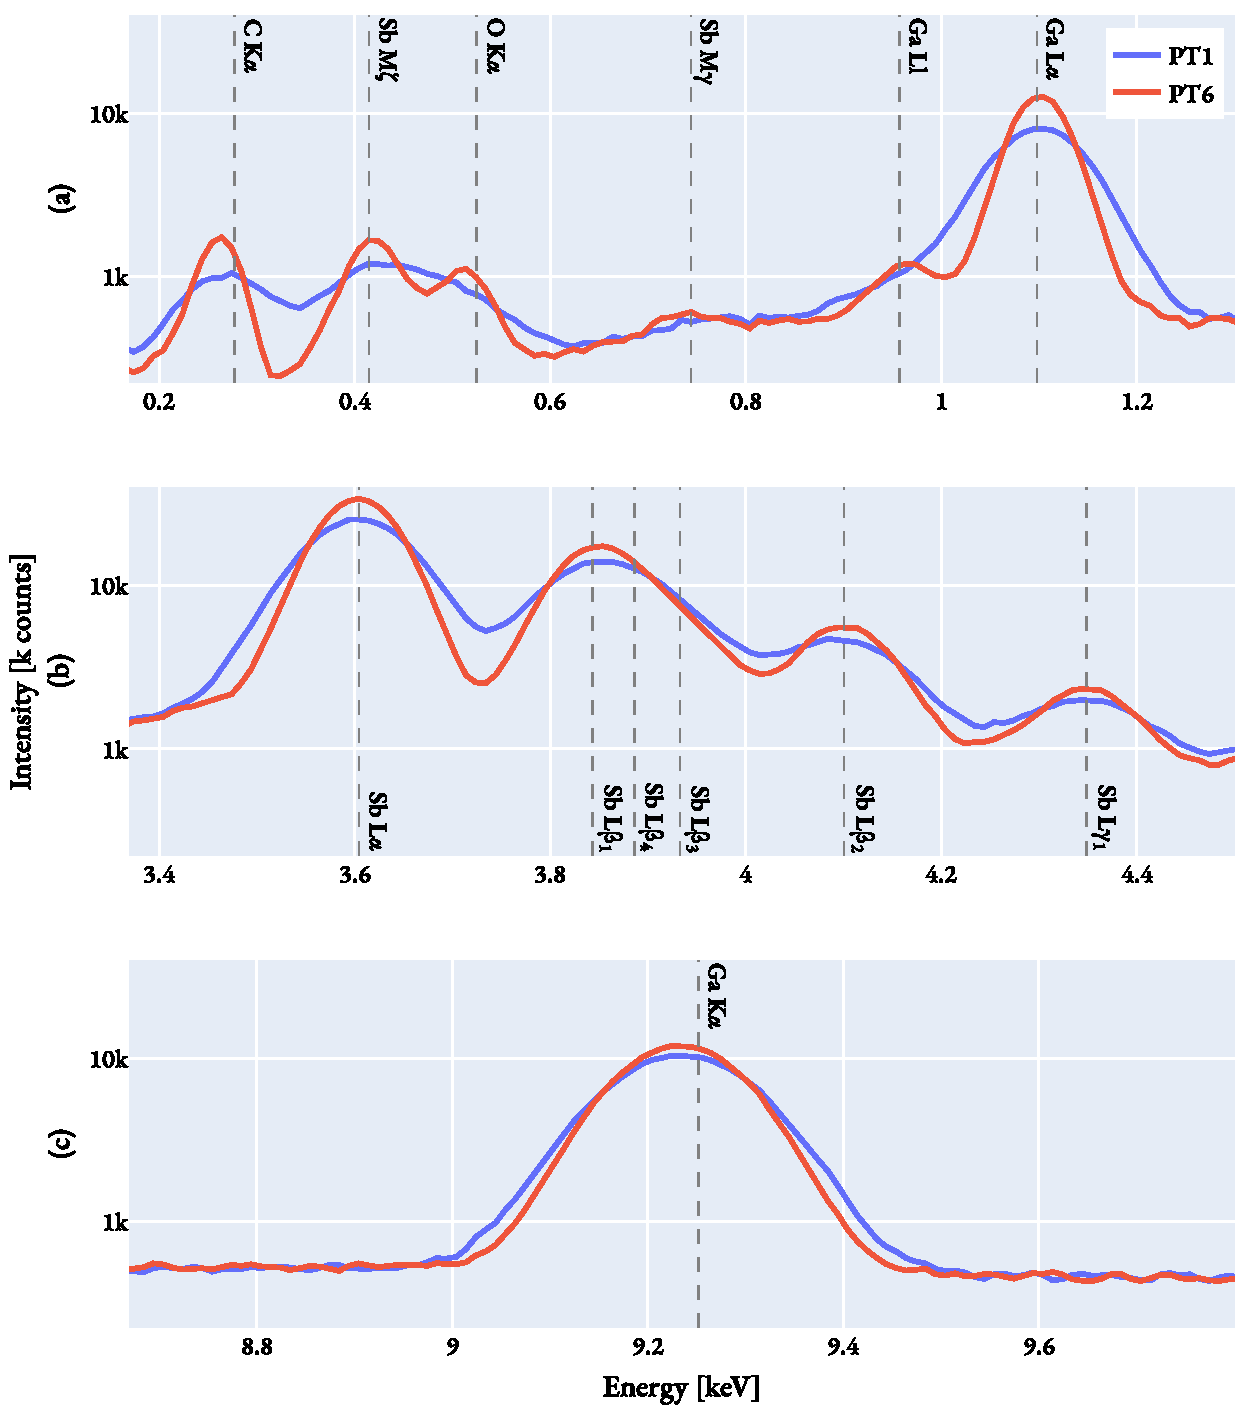
\includegraphics[width=0.95\linewidth]{figures/results/eds_energyResolutions_process_time.pdf}
    \caption{
        Illustration of different energy resolutions on the same specimen, because of different process times.
        The maximum (red) and minimum (blue) process time (PT) on the instrument is used.
        Panel (a) is the spectrum at low energy, where the effect most influential.
        Here both the Sb M$\eta$ and O K$\alpha$, and the Ga Ll and Ga L$\alpha$ are overlapping too much with PT1.
        Panel (b) is the spectrum at medium energy, where the effect less influential.
        Panel (c) is the spectrum at high energy, where the effect is almost negligible.
        All three panels span 1.13 keV and have the same range of counts.
        The vertical lines are the theoretical line energies.
    }
    \label{fig:results:energy_resolutions_process_time}
\end{figure}


The effect of the process time on the FWHM of the lines is shown in \cref{tab:results:PTvsFWHMs}.
The table shows the measured FWHM of Ga L$\alpha$, Sb L$\alpha$, and Ga K$\alpha$ for different process times.
The measurement is done on the Gaussian fit of the peaks.
Additionally, the FWHM of the Mn K$\alpha$ is estimated for each process time.
The table shows the variations on the GaSb specimen with process time (PT) 1, 2, 4, and 6.
The last row shows the FWHM in the GaAs specimen at PT 6 for reference.
All spectra in the table were acquired at 30 kV.
The "*" indicate I$_\textnormal{beam}$ = 400 pA, all other values for I$_\textnormal{beam}$ is 50 pA.


\begin{table}[phtb]
    \begin{center}
        \caption{
            FWHMs of lines with different process times.
            All the FWHMs are in eV, calculated from the Gaussian fit.
            All spectra are acquired at 30 kV and 50 pA.
            GaSb is used as the specimen, except for the last column, where GaAs is used for reference.
        }
        \renewcommand*{\arraystretch}{1.4}
        \label{tab:results:PTvsFWHMs}
        \begin{tabular}{rrrrrr}
            \hline
            \textbf{Line}       & \textbf{PT 1} & \textbf{PT 2} & \textbf{PT 4} & \textbf{PT 6} & \textbf{PT 6, GaAs} \\
            \hline
            %C K$\alpha$&&&&&\\ % C is not it the models used
            Ga L$\alpha$        & 109           & 88            & 73            & 65            & 67                  \\
            Sb L$\alpha$        & 138           & 122           & 108           & 102           & -                   \\
            Mn K$\alpha$ (est.) & 158           & 143           & 132           & 127           & 129                 \\
            Ga K$\alpha$        & 182           & 172           & 165           & 161           & 163                 \\
            \hline
        \end{tabular}
    \end{center}
\end{table}







% 4
\section{Quantitative analysis}
\label{results:data_treatment}


\brynjar{Coming soon. I do observations of AZtec, try out HyperSpy, and make new code which are a step in the right direction (e.g. XPP in a notebook, which is concrete and quantitative.)}





% Old
% % % The model lines

\begin{table}[p]
    \centering
    \caption{
        The lines in the HyperSpy models for the GaAs sample, when As and Ga are added as elements.
        The dashed lines are the lines that are not used in the model, because of low overvoltage.
        HyperSpy differentiates between "X-ray lines" and "Family lines", where the first are the alpha lines of the element.
    }
    \label{tab:results:model_lines}
    \begin{tabular}{c|ccccccccccc}
        X-ray lines  &       &        &       &       &        &       &        &       &       &        \\
        % Model        &       &        &       &       &        &       &        &       &       &        \\
        30 kV        & As Ka & As La  & Ga Ka & Ga La &        &       &        &       &       &        \\
        15 kV        & As Ka & As La  & Ga Ka & Ga La &        &       &        &       &       &        \\
        10 kV        & ----- & As La  & Ga Ka & Ga La &        &       &        &       &       &        \\
        5            & ----- & As La  & ----- & Ga La &        &       &        &       &       &        \\
        \hline
        Family lines &       &        &       &       &        &       &        &       &       &        \\
        30 kV        & As Kb & As Lb1 & As Ln & As Ll & As Lb3 & Ga Kb & Ga Lb1 & Ga Ln & Ga Ll & Ga Lb3 \\
        15 kV        & As Kb & As Lb1 & As Ln & As Ll & As Lb3 & Ga Kb & Ga Lb1 & Ga Ln & Ga Ll & Ga Lb3 \\
        10 kV        & ----- & As Lb1 & As Ln & As Ll & As Lb3 & ----- & Ga Lb1 & Ga Ln & Ga Ll & Ga Lb3 \\
        5  kV        & ----- & As Lb1 & As Ln & As Ll & As Lb3 & ----- & Ga Lb1 & Ga Ln & Ga Ll & Ga Lb3
    \end{tabular}
\end{table}
% \begin{table}[p]
    \centering
    \caption{
        The estimated FWHM of Mn K$\alpha$ with different reference lines.
        When using 'all\_alpha', the alphabetically first line is used as reference.
        That is, for 30 and 15 kV, As K$\alpha$ is used as reference.
        For 10 and 5 kV, As L$\alpha$ is used as reference.
        The original resolution is from the instrument software.
    }
    \label{tab:results:estimated-FWHM}
    \begin{tabular}{ccccc}
        Reference line      & 30 kV & 15 kV & 10 kV & 5 kV  \\
        \hline
        original resolution & 130.0 & 130.0 & 130.0 & 130.0 \\
        \verb|'all_alpha'|  & 138.3 & 148.8 & 132.0 & 132.2 \\
        As Ka               & 137.9 & 146.4 & nan   & nan   \\
        As La               & 130.0 & 130.4 & 131.9 & 132.1 \\
        Ga Ka               & 132.9 & 131.7 & 668.3 & nan   \\
        Ga La               & 129.7 & 130.9 & 127.4 & 130.8
    \end{tabular}
\end{table}
% \subsection{Energy resolution}
% \label{results:resolution}